\section{Prototyp Testplan}
\label{sec:testabnahme}
Überprühfung der Anforderungen.
\subsection{Abnahme-Testplan}
T1. Die Tür bei der Aussensprechstelle muss, nach betätigen der «Türe öffnen» Taste in der Client-App, geöffnet werden können.
\\
\\
T2. In der Client-App wird ein Videosignal von der Kamera der Aussensprechstelleerhalten.
\\
\\
T3. Durch bedienen der Client-App wird ein Audiosignal von der Aussensprechstelle erhalten und umgekehrt.
\\
\\
T4. An der Aussensprechstelle kann man die Namen der Bewohner lesen und auswählen. 
\\
\\
T5. Die Stromversorgung der Anlage wird aus- und dann wider eingeschaltet. Die Anlage muss ohne externen Eingriff wieder Starten.
\\
\\
T6. Mithilfe von Wireshark wird der Netzwerkverkehr analysiert. Der gesamte Datenverkehr aus der Anlage ist verschlüsselt.
\\
\\
T7. Feuchtigkeit, Temperatur und Betriebsbedingungen aus dem Datenblatt mit den Anforderungen vergleichen und überprüfen.
\\
\\  
T8. Durch eine Analyse wird die effektive Auflösung des Videosignals evaluiert. Die Auflösung muss mindestens 720p (ev. 1080p) aufweisen.
\\
\\
T9. Sämtliche Materialkosten zusammenstellen und überprüfen. Die Kosten pro Aussensprechstelle müssen das in den Anforderungen definierte Maximum nicht überschreiten.
\\
\\
T10. Mit bedeckte (Skihandschuh) und/oder nassen Hände muss man bei der Aussensprechstelle Klingeln können. 
\\
\\
T11. Bei der Aussensprechstelle ist nur das Netzwerkkabel zu finden, keine zusätzliche Speisung.
\\
\\
T12. Bei Klingeln und nicht Öffnen der Türe, muss in der Client-App der verpasste Besuch sichtbar sein.
\\
\\
T13. Durch Bedienen der Client-App ist es möglich, frei zu sprechen, ohne dass das Audiosignal an die Aussensprechstelle weitergeleitet wird.
\\
\\
Ergebnisse werden in einer Test-Traceability Matrix visuell festgehalten. Jede Anforderung
wird durch einen Test überprüft. Beziehungsweise, jeder Test verifiziert nur die betroffene Anforderung. Damit werden Überschneidungen vermieden.


\subsection{Resultate}
Bis auf zwei wurden sonst alle Tests bestanden. (\seeref{fig:testmatrix})
\\
Es werden nun die Anforderungen und Tests aufgelistet, welche nicht bestanden wurden.

\subsubsection{Test 12: Verpasste Besuche sind in der Client-App ersichtlich}
Bei Test 12 wird eine Wunschanforderung geprüft: \textit{(W13. Verpasste Besuche sollten
aufgezeichnet werden und in der Client App in Form von einem Foto und Notifikation
sichtbar sein)}. Diese Funktionalität wurde aus Zeitgründen nicht vollständig implementiert. Die Anforderung wurde daher nur teilweise erfüllt. Wenn jemand an der Türe klingelt, wird auf dem mobilen Gerät eine Benachrichtigung angezeigt. Diese Benachrichtigung bleibt solange sichtbar, bis der Benutzer sie gelesen und gelöscht hat. Folgerichtig sind verpasste Besuche trotzdem ersichtlich, auch wenn sie im Web-App nicht erscheinen
\\
Weil es sich um eine Webbapplikation handelt, kann diese Funktionalität ohne grosses Know-How von anderen beteiligten Technologien nachträglich implementiert werden.

\subsubsection{Test 8: Die Auflösung des Videosignales wird evaluiert}
Test 8 prüft zwei Anforderungen. Es handelt dabei um:
\begin{itemize}
	\item A9: Die Kamera für das Videosignal muss eine Auflösung von mind. 1280x720
	Pixel aufweisen. 
	\item W2: Die Kamera für das Videosignal muss eine Auflösung von 1920x1080
	Pixel aufweisen. 
\end{itemize}
Im Nachhinein ist uns klar geworden, dass diese zwei Anforderungen und ihre
dazugehörigen Tests besser definiert werden könnten.
\\
\\
Der Test lautet: \textit{(Durch eine Analyse wird die effektive Auflösung des Videosignales evaluiert. Die Auflösung muss mindestens 720p (oder 1080p) aufweisen.)}
\\
Die eingesetzte Kamera weist effektiv eine Auflösung von 1920x1080 Pixel auf. Das
Problem liegt bei der Digitalisierung des Videosignales. Während der Fachmodul-
Phase wurde die Komplexität der Video-Encoding unterschätzt.
\\
Demzufolge enthält unser System die Hardware, um diese Anforderungen zu
Erfüllen, aber nicht die Rechenkapazität.
\\
Wie im \cref{sec:AussensprechstelleWebapplikation} bereits diskutiert, wäre eine mögliche Lösung der Einsatz einer besseren CPU.

\begin{figure}[htb!]
	\begin{center}
		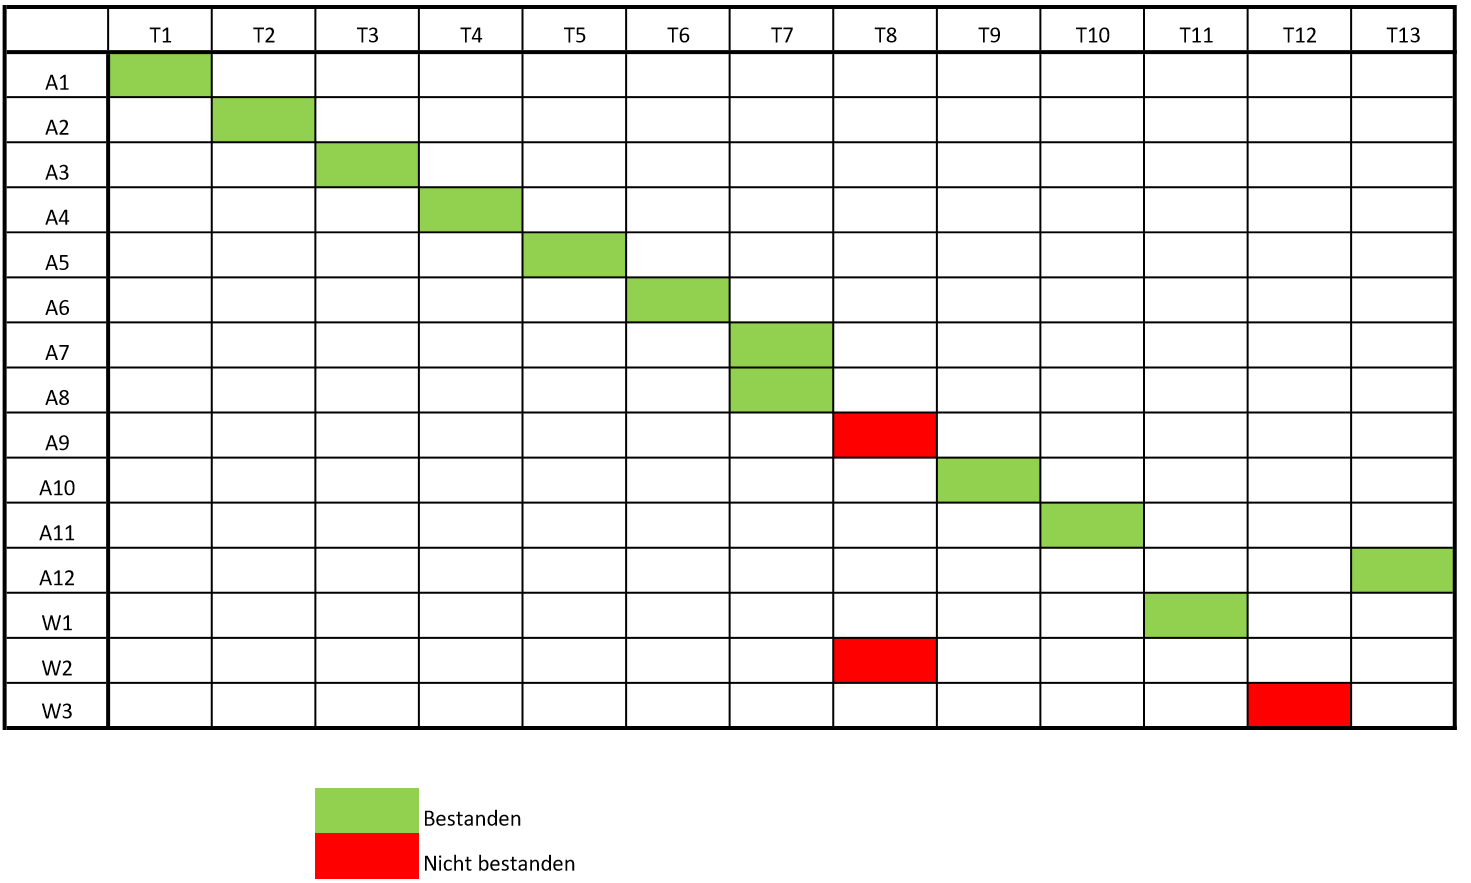
\includegraphics[width=1\textwidth]{testmatrix}
		\caption[Test-Traceability Matrix]{Test Traceability Matrix}
		\label{fig:testmatrix}
	\end{center}
\end{figure}

\newpage